\subsection{Приливы и отливы}

\term{Приливы и отливы}~--- периодические вертикальные колебания уровня океана, являющиеся результатом изменения положения Луны и Солнца. Хотя силы тяготения Солнца почти в 200 раз больше, чем силы тяготения Луны, приливные силы, порождаемые Луной, почти вдвое больше порождаемых Солнцем. Это происходит из-за того, что приливные силы зависят не от величины гравитационного поля, а от степени его неоднородности. Высота приливов зависит от взаимного расположения Луны и Солнца: наибольший~---  силы от Луны и от Солнца действуют вдоль одного направления, а наименьший~--- под прямым углом друг к другу.

\begin{minipage}{.24\tw}
	Ускорение в центре Земли ($T$) определяется формулой \eqref{eq:g}:
	\begin{equation*}
		a_T=\frac{G M}{r^2},
	\end{equation*}
	$M$~--- масса возмущающего тела,
\end{minipage}
\hfill
\begin{minipage}{0.74\tw}
	\vspace{-.5pc}
	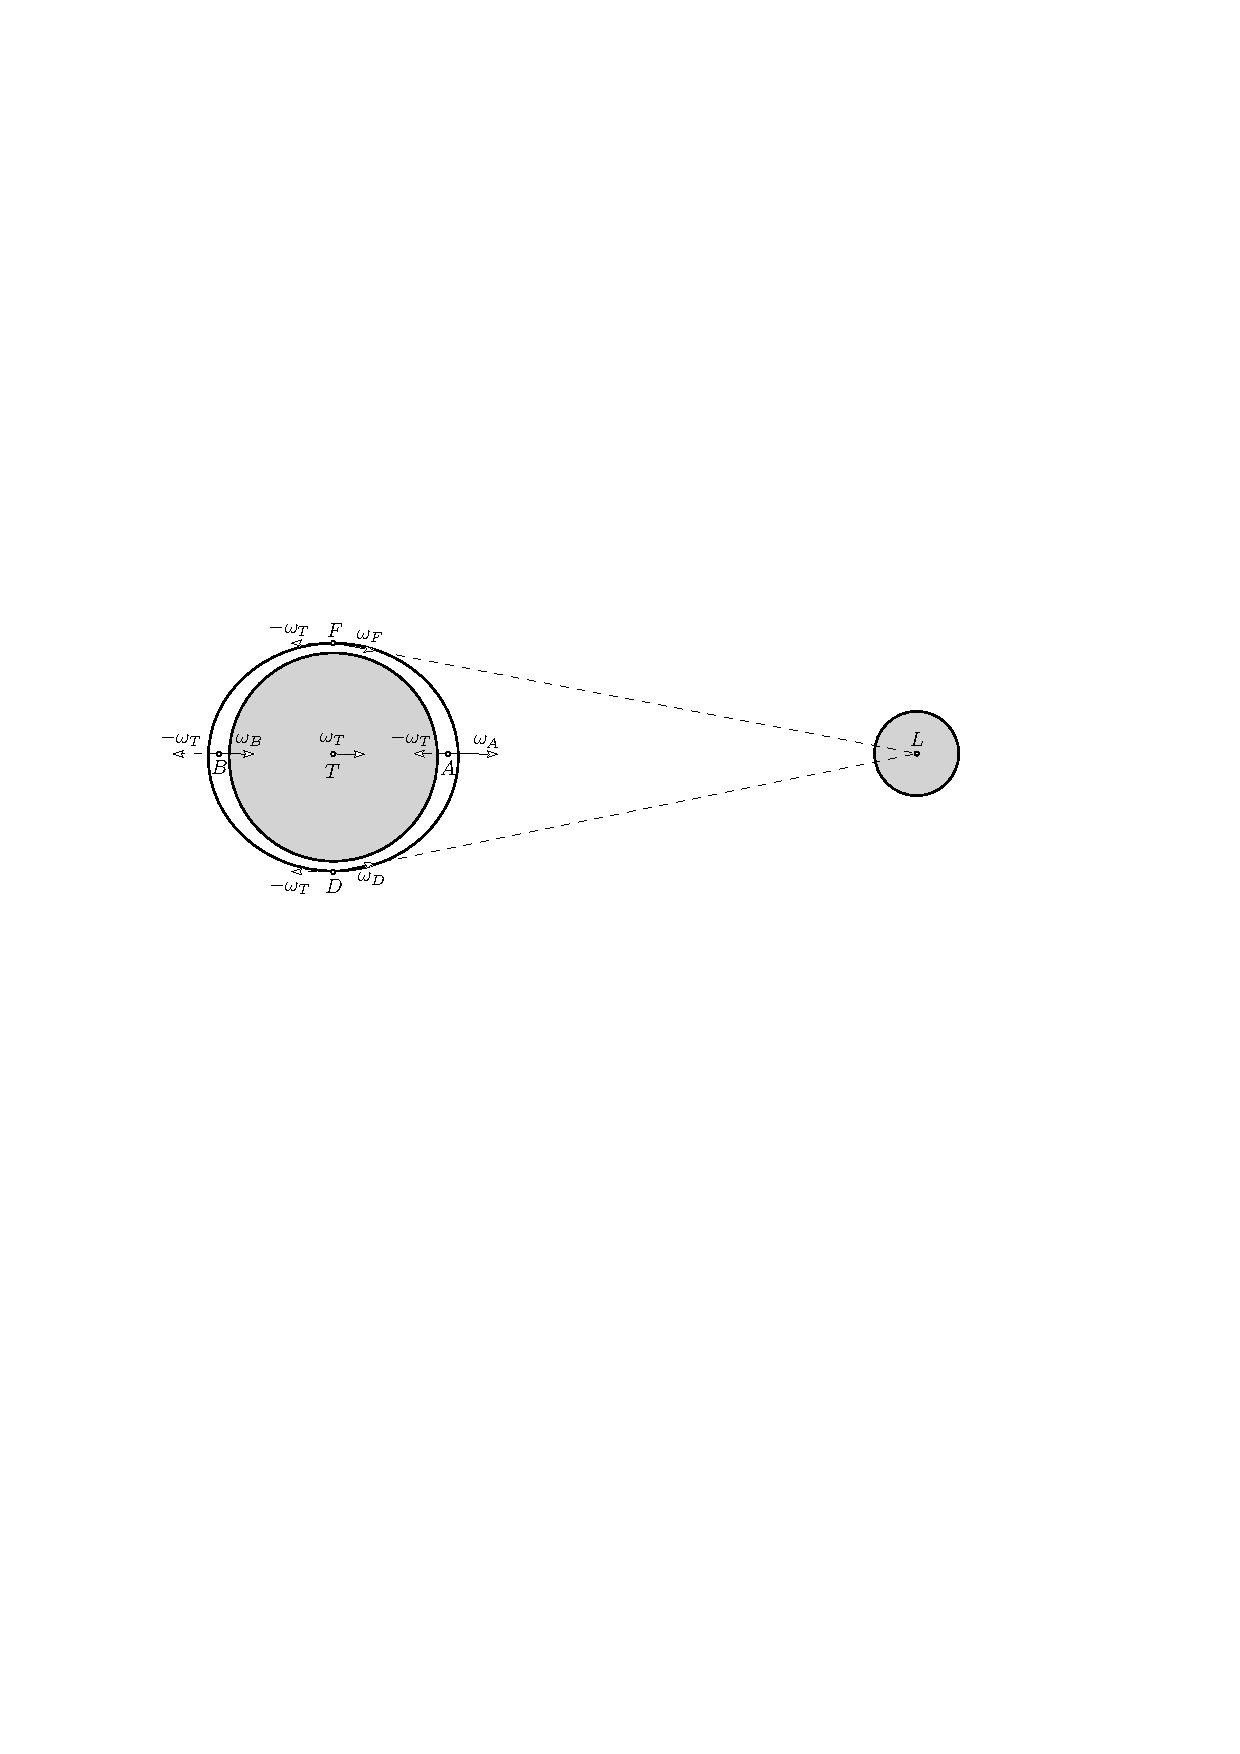
\includegraphics[width = \tw]{Ebb_flow}
	\captionof{figure}{К объяснению приливных сил}\label{Ebb_flow}
\end{minipage}\\[-0.5pc]

$r$~--- расстояние между центрами Земли и данного тела. Аналогично, ускорения в точках $A$ и $B$ равны соответственно
\begin{equation}
	a_A = \frac{G M}{(r - R)^2} \quad \text{и} \quad a_B = \frac{GM}{(r + R)^2},
\end{equation}
где $R$~--- радиус Земли или иного тела, подверженного воздействию приливных сил. Ускорение в точке $A$ относительно точки $T$ равно
\begin{equation}
	a_A - a_T = a_T \cdot \frac{2 r R - R^2}{(r - R)^2} = \frac{GM \left(2 r R - R^2 \right)}{r^2 (r - R)^2} \xrightarrow{R \ll r} \frac{2 G M R}{r^3}.
	\label{eq:ebb-force}
\end{equation}

Под действием лунного притяжения водная оболочка Земли принимает форму
эллипсоида, который вытянут по направлению к Луне. Близ точек $A$ и $B$ будет
прилив, а в точках $F$ и $D$ --- отлив (см.~Рис.\,\ref{Ebb_flow}).
